%!TEX root = paper.tex
Multi-tenancy is not clearly defined, since it has never had an exact and official definition. During the last years, also due to the uprising of cloud applications, multi-tenancy gets researched and used more and more. This can also be seen in figure~\ref{fig:papercount}: all the papers about multi-tenancy referenced in this survey were published after 2005. In this section we discuss various definitions and we shortly describe the various types of multi-tenancy. We also discuss the relationship with the cloud.

\begin{figure}[H]
	\centering
		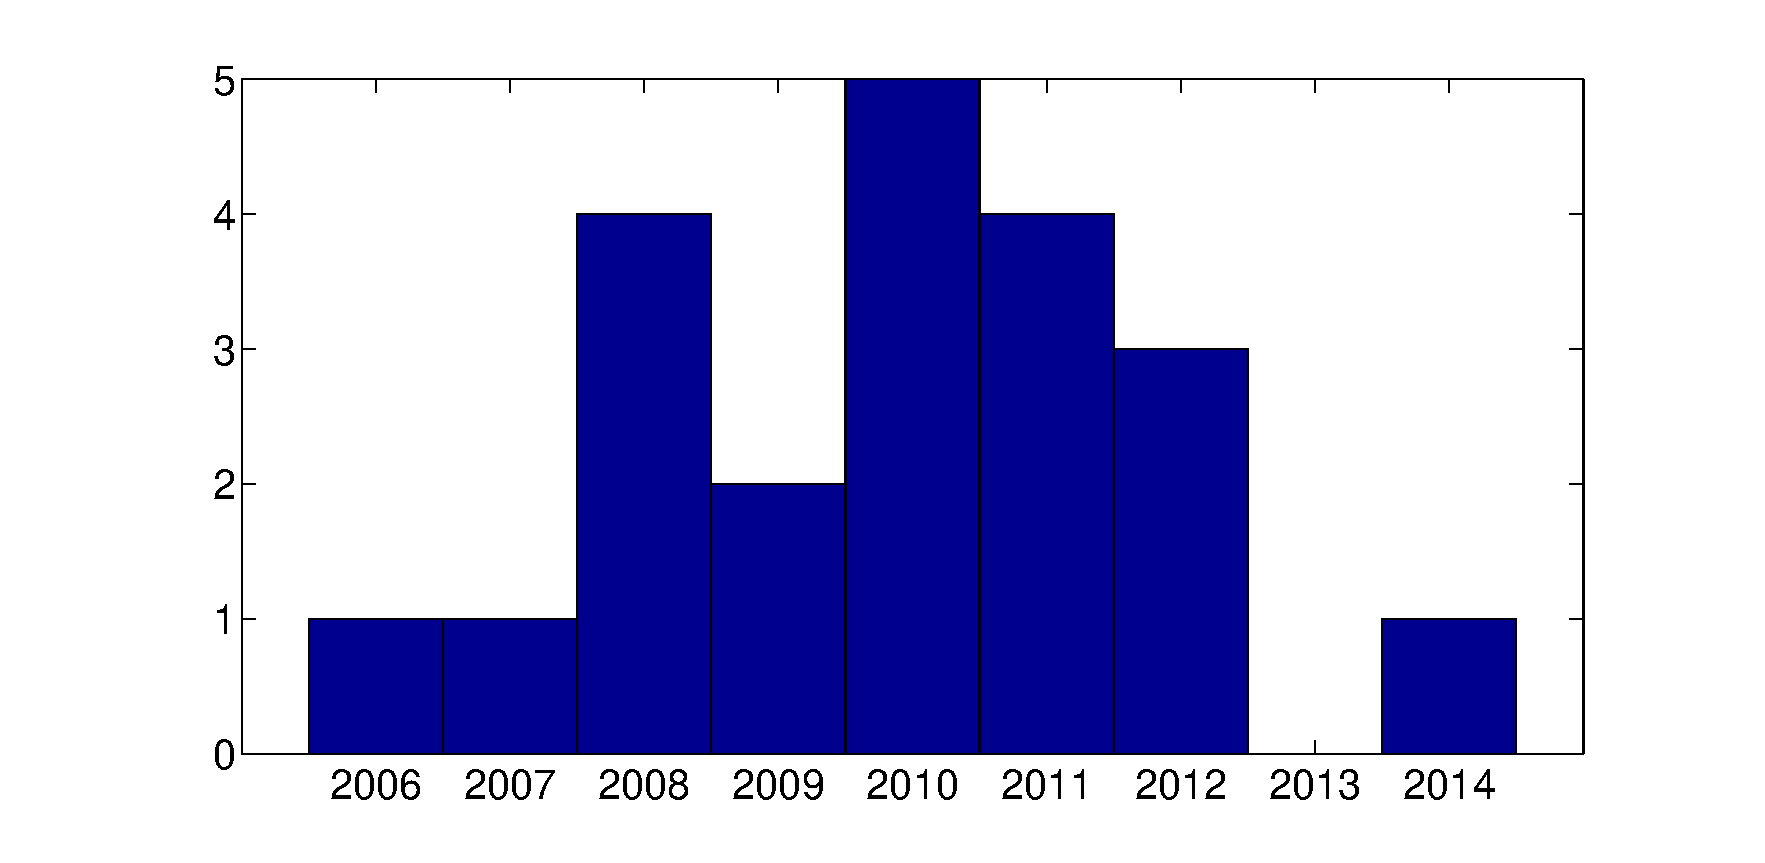
\includegraphics[width=0.5\textwidth]{assets/papers.eps}
		\caption{Number of referenced papers about multi-tenancy, grouped by year}
		\label{fig:papercount}
\end{figure}

\subsection{Definitions}

In multi-tenant research, there are three important concepts: tenants, multi-tenancy and multi-user. In this section we show the variety of definitions of these concepts.

Bezemer and Zaidman~\cite{bezemer2010multi} define a tenant as an organizational entity which rents a multi-tenant \ac{SaaS} solution (where the organization usually groups a number of users). Wang et al.~\cite{wang2008study} have a more loose definition, stating tenants are just different organizations and companies. This definition is also being used by Aulbach et al.~\cite{aulbach2008multi} and Walraven et al.~\cite{walraven2012towards}. Krebs et al.~\cite{krebs2012architecture} have a slightly different definition of tenants: they define it as groups of users that are usually part of different legal entities sharing the same view of an application.

Using this variety of definitions, we can move on to the definitions of multi-tenancy. Wang et al.~\cite{wang2008study} describe multi-tenancy as multiple tenants being ``served concurrently by one or more hosted application instances and databases based on a scalable, shared hardware and software infrastructure''. According to Aulbach et al.~\cite{aulbach2008multi} a multi-tenant architecture is an architecture where multiple tenants are using the same operational system. Walraven et al.~\cite{walraven2012towards} use the definition of Guo et al.~\cite{guo2007framework}, describing it as serving end users from different tenants simultaneously by a single application instance on a shared hardware and software infrastructure. However, Walraven et al. narrow that definition a bit, stating it is an architectural style for especially \ac{SaaS} providers. Krebs et al.~\cite{krebs2012architecture} define multi-tenancy as ``an approach to share an application instance between multiple tenants by providing every tenant a dedicated `share' of the instance''. Bezemer and Zaidman~\cite{bezemer2010multi} define a multi-tenant application as one shared application and database instance to multiple tenants, using shared hardware resources.

There is a difference between multi-tenant applications and multi-user applications. This is made clear by Bezemer and Zaidman~\cite{bezemer2010multi}: They define a multi-user application as an application in which \emph{all} users use the same application with limited configuration options, whereas a multi-tenancy application groups the users per tenant. A multi-tenancy application additionally has more configuration options. The similarity in both models is that users are using a shared application. % Extra citaties??

From the variety of definitions above it can be concluded that there still is not an exact definition of multi-tenancy. The reoccurring elements in almost all these definitions are that tenants are organizations or companies, and that multi-tenancy means that multiple tenants are using the same system. The definition of multi-user is unambiguous and means all users are using the same application, without grouping the users into organizations. In the following section we will elaborate on the different types of multi-tenancy. 

\subsection{Different types of multi-tenancy}

There are three main levels of multi-tenancy, as described by Chong et al.~\cite{chong2006multi} and Bezemer and Zaidman~\cite{bezemer2010multi}:
\begin{compactenum}
\item shared application with a separated database
\item shared application with a shared database (separate schema)
\item shared application with a shared schema
\end{compactenum}
They consider the latter as pure multi-tenancy. Lin et al.~\cite{lin2009feedback} and Aulbach et al.~\cite{aulbach2009comparison} agree on this, sometimes calling it \emph{native} multi-tenancy. Guo et al.~\cite{guo2007framework} also mention native multi-tenancy, but they leave out the database. Krebs et al.~\cite{krebs2012architecture} use the \emph{affinity} and \emph{persistency} concepts: affinity describes which server(s) handle which tenant(s) and persistency describes the way of usage of the database (shared or separated). These concepts can easily be translated into the levels of Bezemer and Zaidman~\cite{bezemer2010multi}. 

A fourth level of multi-tenancy (as described by Guo et al.~\cite{guo2007framework}) is the multiple instances pattern. This means each tenant has its own dedicated instance of the application, running on shared hardware.

Guo et al.~\cite{guo2007framework} suggest the implementation of a multi-tenancy enablement layer. This should create a separation between usage and resources, creating the required isolations and allowing customizations. This can be compared to the blueprint of Bezemer and Zaidman~\cite{bezemer2010multi}, since both approaches should have little impact on the single-tenant code.

\subsection{Multi-tenancy vs. the cloud}

Multi-tenancy has a relationship with the cloud, but that does not imply they are the same. For example, a multi-tenant application does not have to run in the cloud and a cloud application does not have to be multi-tenant. In this section we explain this relationship.

Firstly, there are various service models for cloud services, as discussed by Dillon et al.~\cite{dillon2010cloud}:
\begin{compactenum}
\item \acf{SaaS} (example: Google Mail/Docs)
\item \acf{PaaS} (example: Google AppEngine)
\item \acf{IaaS} (example: Amazon EC2)
\item \acf{DaaS} (example: Google BigTable)
\end{compactenum}

According to them, multi-tenancy has a close relationship with the \ac{SaaS} domain, because multi-tenancy gains the most benefits within this model. Tsai et al.~\cite{tsai2010towards} go even further, stating \ac{SaaS} ``is characterized by its multi-tenancy architecture''. 

Dillon et al.~\cite{dillon2010cloud} also describe the several essential characteristics of cloud services, including resource pooling (`pooling' computing resources together in an effort to serve multiple consumers) and rapid elasticity (the consumption of resources can rapidly increase and the usage is not predictable upfront). These are both challenges that also exist for multi-tenant applications, as mentioned by Krebs et al.~\cite{krebs2012architecture} and Bezemer and Zaidman~\cite{bezemer2010multi}.

In the following sections we discuss the current state of research on multi-tenancy. We do so by discussing the main challenges of multi-tenancy, namely Security, Scalability, \ac{QoS} and Variability. For each subject we describe what it means and how it can be achieved in the context of multi-tenancy. We also address the points of interest for future research.